\subsubsection{Learning from Observation}

\begin{figure}[t]
    
    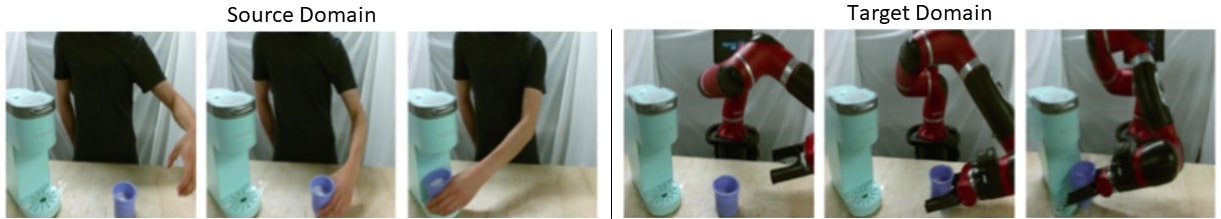
\includegraphics[width=\textwidth]{figures/images/embodiment_mismatch/embo.jpg}
    \caption{Representation of \textbf{embodiment mismatch problem}. (Left) The source domain
    represented by a video of human performing a task. (Right) The target domain, represented
    by the robot that executes the observed task.}
    \label{fig:embo_mismatch}
    
\end{figure}

\label{sec:lfo}
In the previous sections, the methodologies assumed access to the agent actions, working with state-action trajectories. In \textit{Learning from Observation} (LfO), this assumption is relaxed, and methods for learning from \textbf{state-only} demonstrations are introduced. This approach has gained significant attention in recent years~\cite{torabi2019recent_advances_lfo} because it theoretically enables a robotic system to be programmed as naturally as possible. Ideally, a robotic system should be able to replicate a task by observing a human or another robot performing it, without access to the actions taken, in contrast to the methods described thus far.

To address this problem, several questions need to be answered:

\begin{enumerate}
\item How can embodiment mismatches be resolved when the demonstrator has a different embodiment than the imitator?
\item How can the correspondence problem be handled when the demonstrator viewpoint differs from the imitator?
\item Once the perception subsystem issues are resolved, how is the policy $\pi^{L}$ obtained?
\end{enumerate}

The first question refers to the \textit{correspondence problem} introduced in Section~\ref{sec:sod}. This problem arises when the demonstrator embodiment differs from that of the learner, meaning that methods cannot directly use the recorded trajectories of the demonstrator.

One approach to solving this problem is to use methods that perform \textit{image-to-image} translation. This involves using generative deep architectures to transform images of a subject in one domain (e.g., a human demonstrator) into images where the context remains the same, but the subject is different (e.g., the human demonstrator is replaced by the target robot) as depicted in Figure \ref{fig:embo_mismatch}. This approach has been followed by authors in \cite{smith2019avid,xiong2021learning_by_watching,li2021meta_watching_video_demonstration}.

Specifically, the authors in \cite{smith2019avid, xiong2021learning_by_watching} used the Cycle-GAN architecture \cite{zhu2017cycle_gan} to translate images from the source domain (human images) to the target domain (robot images) in an unsupervised manner. The work in \cite{zhu2017cycle_gan} shifted the translation problem from a paired image setting, where each source domain image has a corresponding target domain image, to an unpaired image setting, where the source domain image does not have a corresponding target domain image.

To address this, Cycle-GAN introduces a novel learning procedure involving two translation models: $G: X \rightarrow Y$ and $F: Y \rightarrow X$. The first model maps inputs from the source domain to the target domain, while the second model maps inputs from the target domain back to the source domain. These two models are trained in an adversarial setting by minimizing the loss function shown in Formula \ref{eq:cycle_gan_loss}.
\begin{equation}
    \label{eq:cycle_gan_loss}
    \begin{aligned}
        \mathcal{L}(G,F,D_X,D_Y) &= \mathcal{L}_{GAN}(G,D_Y,X,Y) + \\
        &\quad \mathcal{L}_{GAN}(F,D_X,Y,X) + \lambda\mathcal{L}_{cyc}(G,F) 
        \\ \\
        \mathcal{L}_{GAN}(Z,D_{K},S,T) &= \mathbb{E}_{t \sim p_{data}(t)}\left[ \log(D_K(t)) \right] + \\
        &\quad \mathbb{E}_{s \sim p_{data}(s)}\left[ \log(1 - D_K(Z(s))) \right]    
        \\ \\
        \mathcal{L}_{cyc}(G,F) &= \mathbb{E}_{x \sim p_{data}(x)}\left[ \|F(G(x)) - x\|_{1} \right] +  \\
        &\quad \mathbb{E}_{y \sim p_{data}(y)}\left[ \|G(F(y)) - y\|_{1} \right]
        \end{aligned}
\end{equation}

Here, $\mathcal{L}_{GAN}$ is the adversarial loss component, where the discriminator $D_{K}$ is trained to distinguish between real samples $t \in T$ and translated samples $Z(s)$. The generator $Z$ is trained to generate samples that are as similar as possible to those in the target domain, starting from samples in the source domain. Meanwhile, $\mathcal{L}_{cyc}$ is a loss term that aims to maintain consistency between the generated samples and the ground truth one.

The application of this concept in the domain of interest, lead to a dataset for the source domain was composed of human demonstrations as well as a small amount of ``random" data, in which the human moves around the scene but does not specifically attempt the task, while for the target domain, it consists of robot images executing randomly sampled actions in a few different settings.

The second question also addresses a variant of the correspondence problem, where, in addition to the embodiment mismatch, the problem of \textit{different viewpoints} is also encountered (Figure \ref{fig:time_contrastive}). This issue has been tackled in \cite{sermanet2018time_contrastive, liu2018imitation_from_observation}.

In \cite{sermanet2018time_contrastive}, a Convolutional Neural Network was trained using a \textit{Triplet-Loss} \cite{schroff2015triplet_loss}. The aim was to train a network to predict an embedding independent of the viewpoint, but containing only task-relevant features. To achieve this, the network had to produce an embedding, $f(x)$, such that $|| f(x^{a}_{i}) - f(x^{p}_{i})||^{2}_{2} + \alpha < || f(x^{a}_{i}) - f(x^{n}_{i})||^{2}_{2}$ for all $(f(x^{a}_{i}), f(x^{p}_{i}), f(x^{n}_{i})) \in \mathcal{T}$, where $\mathcal{T}$ is the set of all possible triplets in the dataset. This implies that embeddings produced by samples from different viewpoints, but sharing the same time-step, $(x^{a}_{i},x^{p}_{i})$, should be similar, while embeddings produced by samples from the same viewpoint, but at different time-steps, $(x^{a}_{i},x^{n}_{i})$, should be different (Figure \ref{fig:time_contrastive}).

In \cite{liu2018imitation_from_observation}, a different approach was employed. Here, a \textit{context translation problem} was addressed using an Encoder-Decoder architecture (Figure \ref{fig:context-translation}). The proposed architecture was trained on pairs of demonstrations, $\mathcal{D}_{i}=[o^{i}_{0},o^{i}_{1},\dots,o^{i}_{T}]$ and $\mathcal{D}_{j}=[o^{j}_{0},o^{j}_{1},\dots,o^{j}_{T}]$, composed of visual observations. Samples in $\mathcal{D}_{i}$ come from the source context $\omega_{i}$, while samples in $\mathcal{D}_{j}$ come from the target context $\omega_{j}$. The model must output the observations in $\mathcal{D}_{j}$ conditioned on both $\mathcal{D}_{i}$ and the first observation $o^{j}_{0}$ from the target domain.

As will be explained next, the outputs of both the Time-Contrastive and the Context-Translation networks can be used to obtain an engineered reward function.

\begin{figure}[t]
    \centering
    \begin{subfigure}[b]{0.50\textwidth}
        \centering
        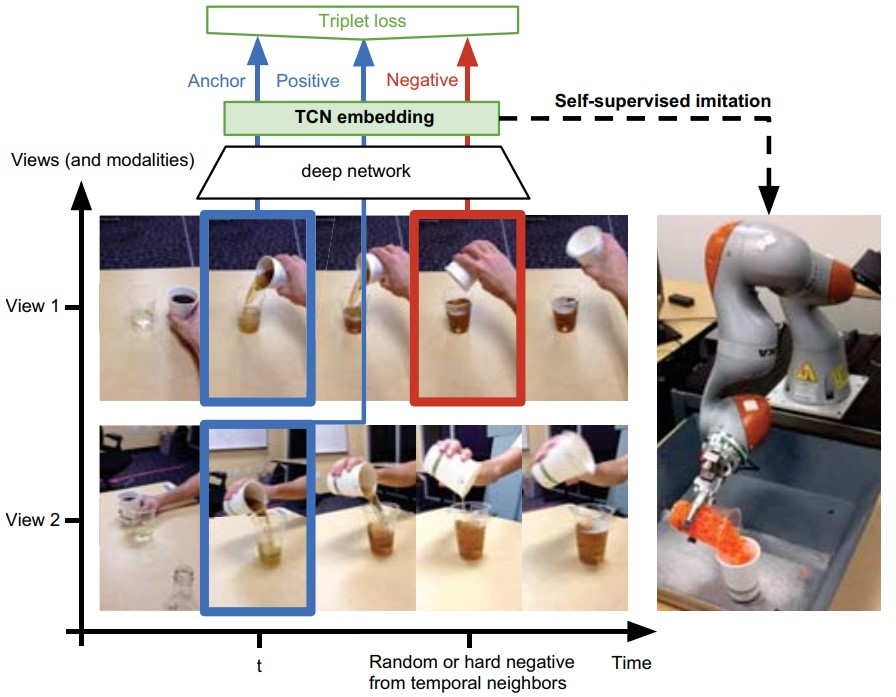
\includegraphics[width=\textwidth]{figures/images/view_point_mismatch/time-contrastive-network.jpg}
        \caption{\textit{Time-Contrastive network}, proposed in~\cite{sermanet2018time_contrastive}.}
        \label{fig:time_contrastive}
    \end{subfigure}
    \hfill
    \begin{subfigure}[b]{0.45\textwidth}
        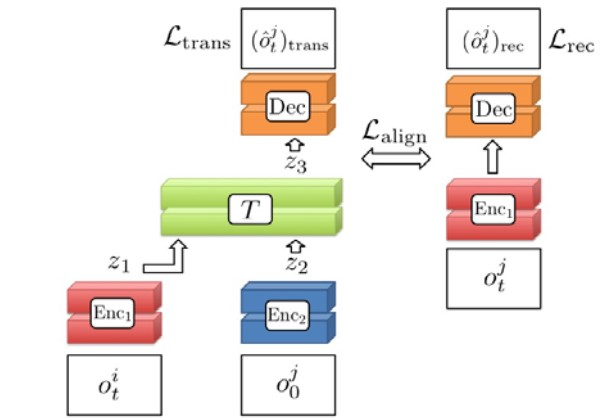
\includegraphics[width=\textwidth]{figures/images/view_point_mismatch/context-translation-model.jpg}
        \caption{\textit{Context-Translation network}, proposed in~\cite{liu2018imitation_from_observation}}
        \label{fig:context-translation}
    \end{subfigure}
    \caption{Examples of how the mismatch between demonstrator viewpoint and learner viewpoint can be handled.}
    \label{fig:differet_viewpoint}
\end{figure}


The third question concerns the method by which the final learned policy is derived. To present the different approaches, it is essential to distinguish between \textit{Model-Free} and \textit{Model-Based} methods (Figure \ref{fig:lfo_taxonomy}).

\begin{figure}[t]
    
    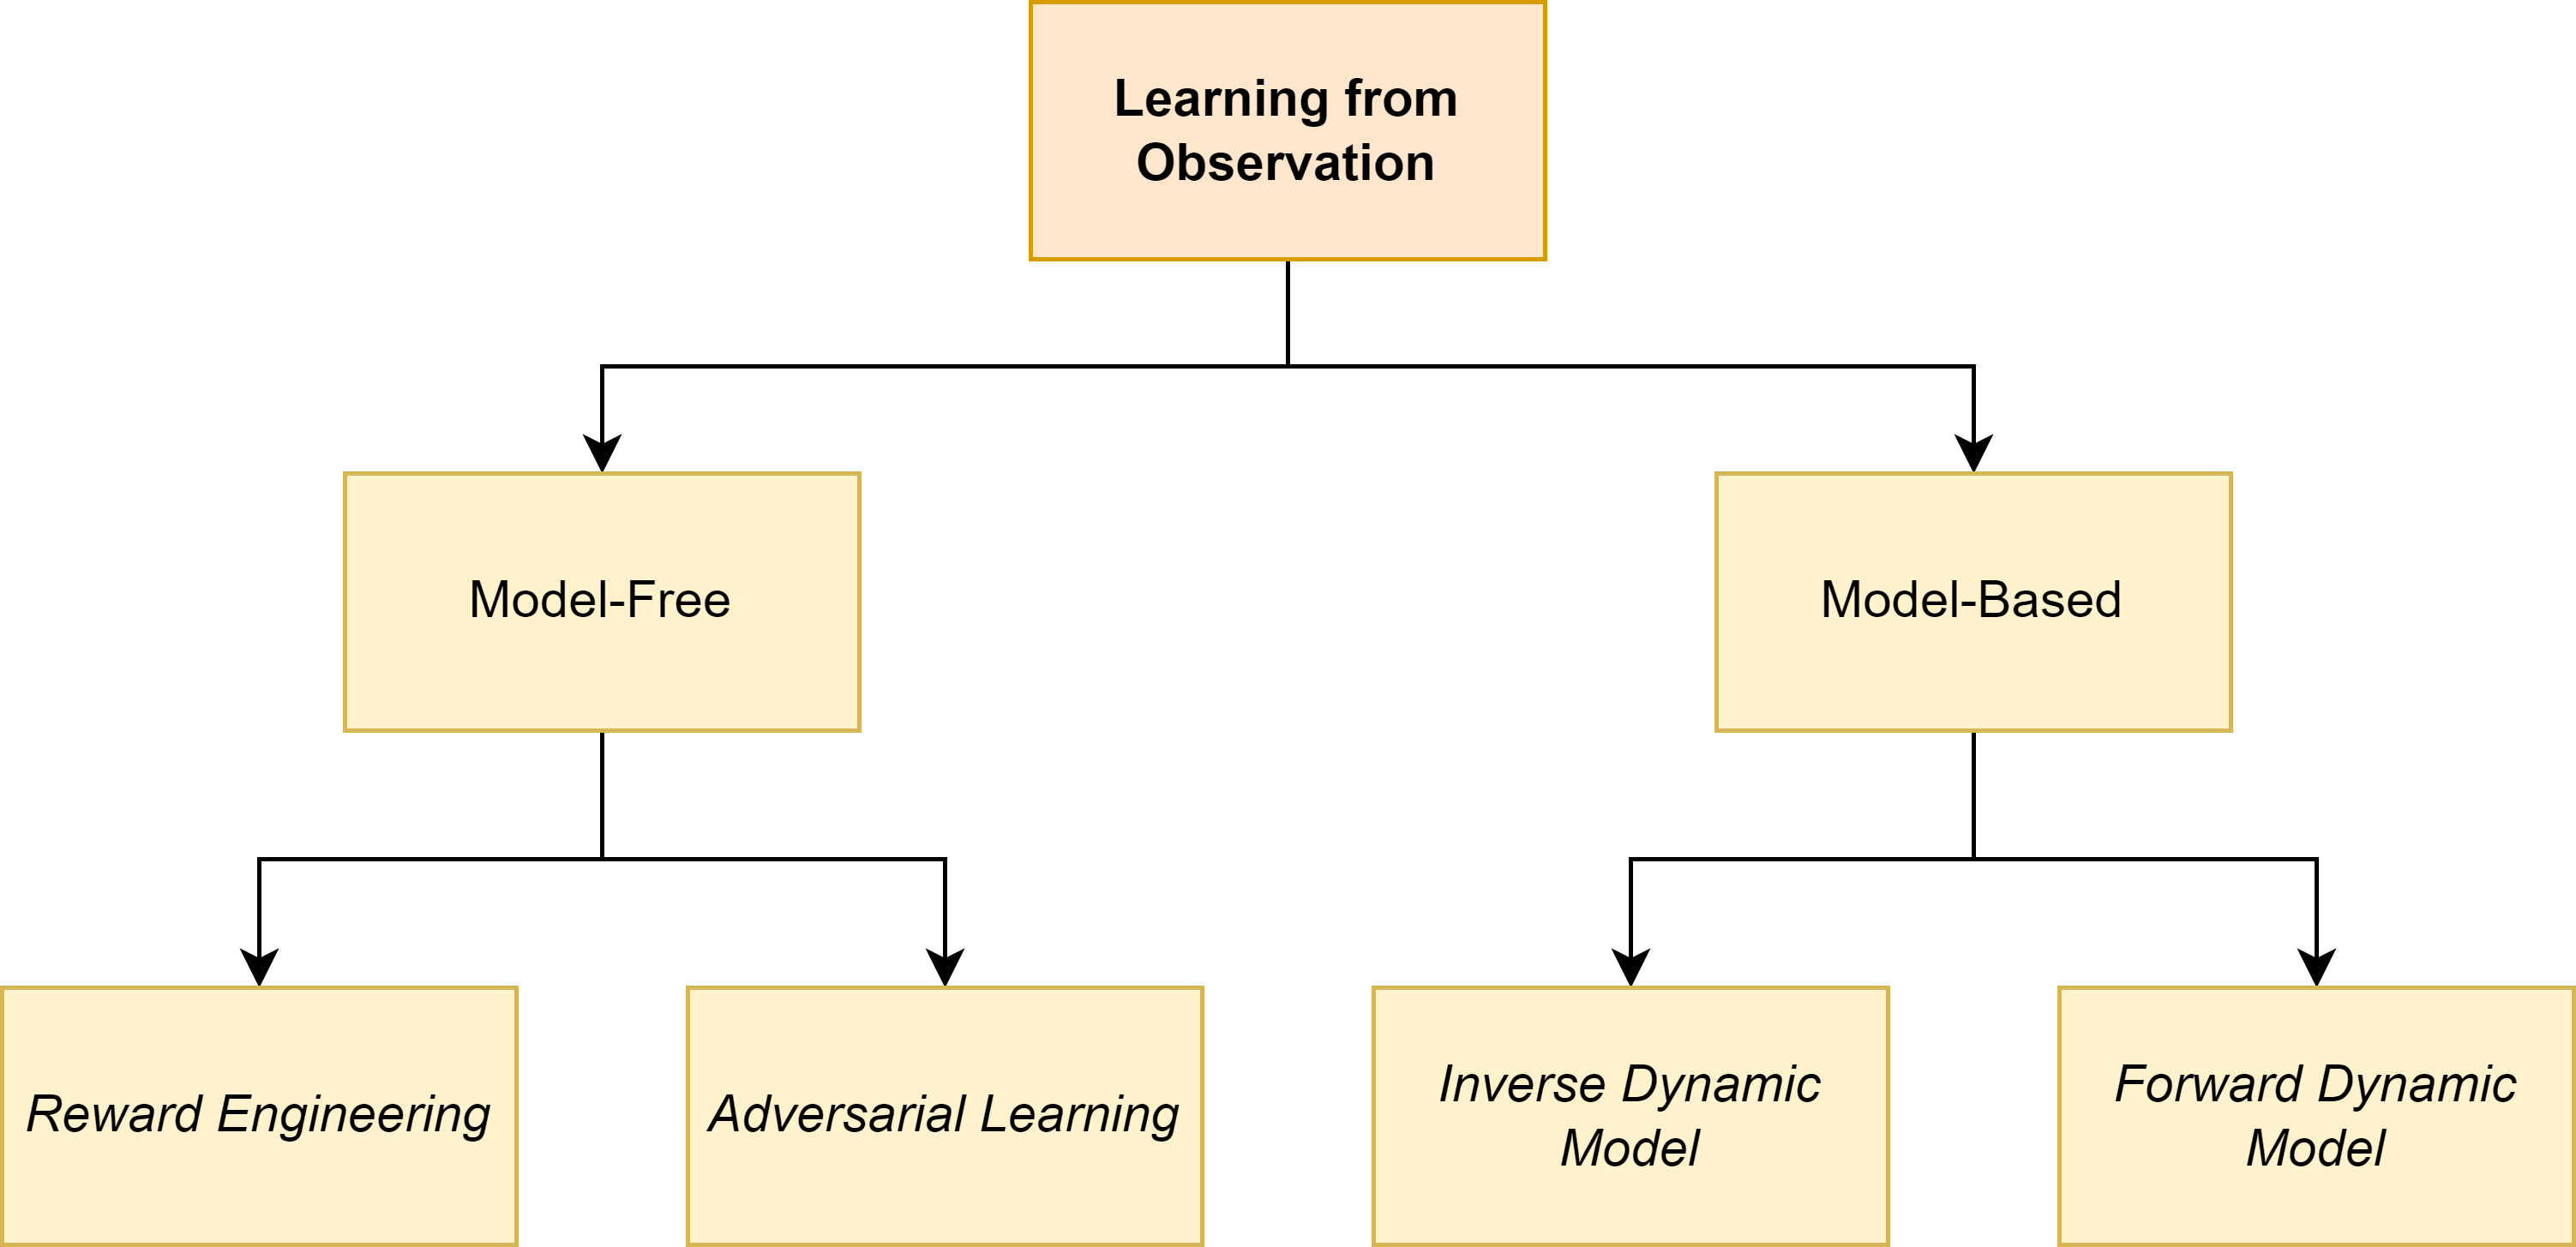
\includegraphics[width=0.8\textwidth]{figures/images/lfo_taxonomy.png}
    \caption{Learning from Observation taxonomy}
    \label{fig:lfo_taxonomy}
    
\end{figure}


\paragraph*{Model-Free}\mbox{}\\
Model-Free methods are characterized by the fact that they do not leverage knowledge about the environment dynamics, which can either be given a priori or learned through data-driven approaches. A further classification must be done between \textit{Reward Engineering} and \textit{Adversarial Learning} approaches.

\textbf{Reward Engineering} methods are characterized by the use of a hand-designed reward function to train the policy according to the Reinforcement Learning paradigm \cite{sutton2018reinforcement}. Methods based on this approach include \cite{liu2018imitation_from_observation,sermanet2018time_contrastive,xiong2021learning_by_watching,zakka2022xirl}.

In \cite{liu2018imitation_from_observation}, the reward function is defined as in Formula \ref{eq:liu2018imitation_from_observation_reward}.
\begin{equation}
    \label{eq:liu2018imitation_from_observation_reward}
    \begin{aligned}
        R(o^{l}_{t}) = -\left\|Enc_{1}(o^{l}_{t}) - \frac{1}{n} \sum_{i=1}^{n}F(o_{t}^{i},o_{0}^{l})\right\|^{2}_{2} - \\ w_{rec} \left\|o^{l}_{t} - \frac{1}{n} \sum_{i=1}^{n}M(o_{t}^{i},o_{0}^{l})\right\|^{2}_{2}
    \end{aligned}
\end{equation}
The first term is the classic Feature Tracking reward function, which aims to minimize the Euclidean Distance between the encoding of the current learner observation $o^{l}_{t}$ and the encoding of the demonstration in the learner context. The second term penalizes the policy for experiencing observations that differ from the translated observation.

In \cite{sermanet2018time_contrastive}, the reward function is defined according to Formula \ref{eq:sermanet2018time_contrastive_reward}.
\begin{equation}
    \label{eq:sermanet2018time_contrastive_reward}
    \begin{aligned}
        R(\textbf{v}_{t}, \textbf{w}_{t}) = - \alpha \left\| \textbf{w}_{t} - \textbf{v}_{t} \right\|^{2}_{2} - \beta \sqrt{\gamma + \left\| \textbf{w}_{t} - \textbf{v}_{t} \right\|^{2}_{2}}
    \end{aligned}
\end{equation}
Where $\textbf{v}_{t}$ is the TCN embedding of the video demonstration at timestep $t$, and $\textbf{w}_{t}$ is the TCN embedding produced by the robot observation (Figure \ref{fig:time_contrastive}).

In \cite{xiong2021learning_by_watching}, a \textbf{keypoint-representation} (Figure \ref{fig:lbw}) is obtained for both the current robot observations $z_{t}$ and each frame of the translated demonstration video $\{z^{E}_{p}\}_{p=1}^{T}$. The reward is then computed as in Formula \ref{eq:xiong2021learning_by_watching_reward}.
\begin{equation}
    \label{eq:xiong2021learning_by_watching_reward}
    \begin{aligned}
        R(z_{t},z_{t+1},z^{E}) = - \lambda_{1} \min_{p} \left\|z_{t}-z^{E}_{p}\right\| - \\ \lambda_{2} \min_{p} \left\|(z_{t+1}-z_{t}) - (z^{E}_{p+1}-z^{E}_{p})\right\|
    \end{aligned}
\end{equation}
The main idea is to generate actions that minimize the distance between the translated keypoints and the keypoints obtained from the current robot observation, thereby reproducing the demonstrated trajectory. The \textit{min} operator is necessary because the robot and the demonstration are not temporally aligned; there is no a priori knowledge about which demonstration frame corresponds to the current agent state.

\begin{figure}[t]
    \centering
    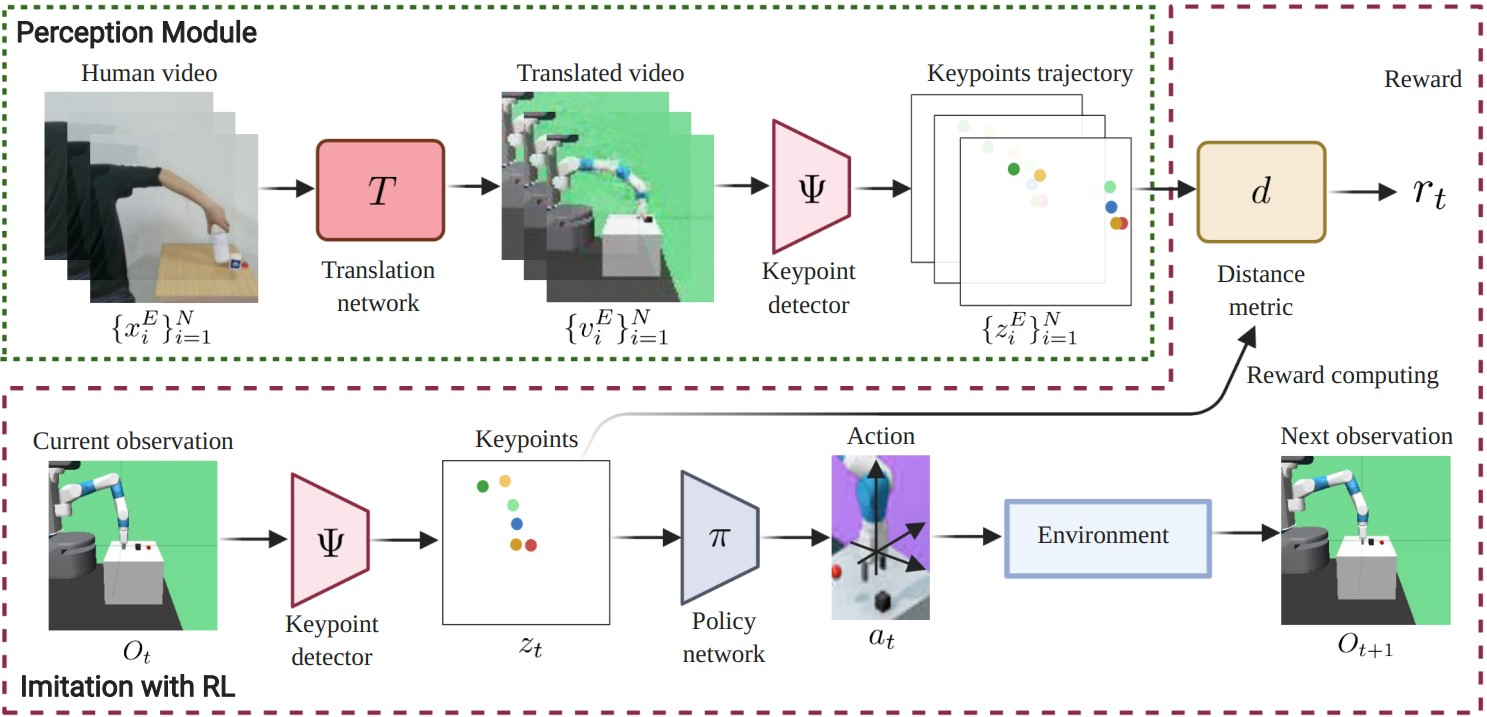
\includegraphics[width=0.8\textwidth]{figures/images/learning_by_watching/learning_by_watching.jpg}
    \caption{Architecture proposed by~\cite{xiong2021learning_by_watching}.}
    \label{fig:lbw}
\end{figure}

In \cite{zakka2022xirl}, the reward function was defined as $R(s_{t}) = -\frac{1}{k} \ || \phi(s_{t}) - g||^{2}_{2}$, where $g$ is the goal embedding, defined as the mean embedding of the last frame of all the demonstration videos in the dataset, while $\phi(s_{t})$ is the embedding of the current observation. Experimental results, on simulation data proved that the proposed method can be used to learn tasks from cross-embodiment demonstrations, outperforming baseline \cite{sermanet2018time_contrastive} in terms of both sample efficiency and performance.


\paragraph*{Adversarial Learning} methods rely on the Adversarial Learning paradigm and are closely related to the GAIL methods (Section \ref{sec:gail}). Unlike the methods discussed in the GAIL section, these methods do not assume access to the demonstrator's actions. Preliminary works in this area have been proposed in \cite{merel2017learning,torabi2018gaifo}.

The goal of authors in \cite{merel2017learning} was to demonstrate that the Adversarial Learning setting can be effectively used even without action information. To test this hypothesis, the authors conducted a series of experiments in simulation for a walking task, where the same RL policy was trained in two contexts: one where the Discriminator had access to the (state, action) pair, and another where the Discriminator had access to state-only demonstrations. The results showed no substantial difference between the two settings, supporting the hypothesis that the essential information for task learning is contained in the state.

\begin{algorithm}[t]
\caption{GAIfO algorithm \cite{torabi2018gaifo}}
\label{alg:gaifo_algorithm}
\begin{algorithmic}
\REQUIRE Initial policy $\pi^{L}_{\phi}$, Initial Discriminator $D_{\theta}$
\REQUIRE State-only expert demonstration trajectories $\tau^{E} = \left \{ (s,s') \right \}$
\WHILE {Policy Improves}
    \STATE Execute $\pi^{L}_{\phi}$ and collect state transitions $\tau^{L} = \left \{ (s,s') \right \}$
    \STATE Update $D_{\theta}$, with $\mathcal{L}_{D_{\theta}} = - \ ( \ \mathbb{E}_{\tau^{L}}[\log (D_{\theta}(s, s')) ] + \mathbb{E}_{\tau^{E}}[\log(1 - D_{\theta}(s, s'))] \ )$
    \STATE Update $\pi^{L}_{\phi}$, with reward $ r_{\pi^{L}_{\phi}} = - \ ( \ \mathbb{E}_{\tau^{L}}[\log(D_{\theta}(s, s'))] \ )$
\ENDWHILE
\end{algorithmic}
\end{algorithm}

The next significant work was proposed by the authors of \cite{torabi2018gaifo}, who formalized the \textit{GAIfO} algorithm (Algorithm \ref{alg:gaifo_algorithm}), an extension of GAIL \cite{ho2016gail} to state-only demonstrations. The proposed algorithm was used to train a network to solve tasks in a simulation environment \cite{brockman2016openai}, with both low-dimensional state representation and visual-state representation. Results regarding the number of demonstrated trajectories are reported in Figure \ref{fig:gaifo_results}.

As noted from the results, GAIfO outperforms previous observation-based methods \cite{sermanet2018time_contrastive,torabi2018bco} in settings with a low number of expert trajectories. The main drawback of GAIfO is the \textbf{high number of environmental interactions} needed to learn a policy, as it uses the model-free TRPO \cite{schulman2015trpo} algorithm. This issue was addressed by DEALIO \cite{torabi2021dealio}, which replaced the model-free algorithm with PILQR \cite{chebotar2017pilqr}, a model-based RL algorithm discussed next.

\begin{figure}[tb]
     \centering
     \begin{subfigure}[b]{0.8\textwidth}
        \centering
         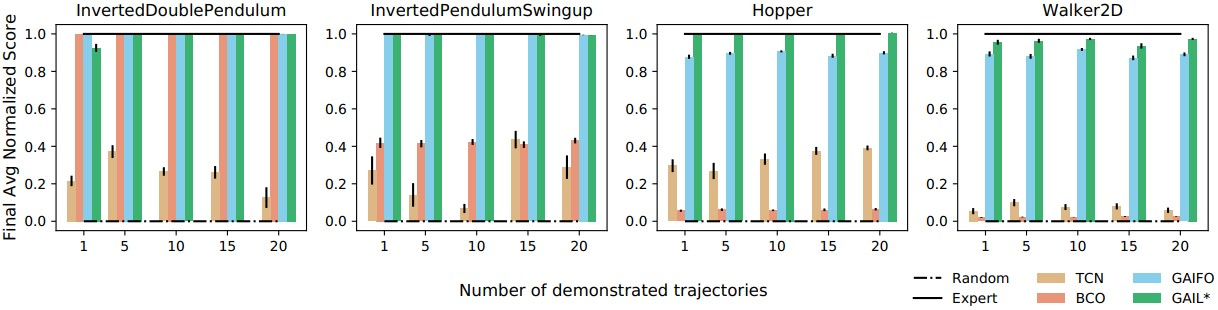
\includegraphics[width=\textwidth]{Figures/images/gaifo_results/gaifo_results.jpg}
         \caption{Experimental results in low-dimensional state space}
         \label{fig:low_dimensional}
     \end{subfigure}
     \vfill
     \begin{subfigure}[b]{0.8\textwidth}
        \centering
         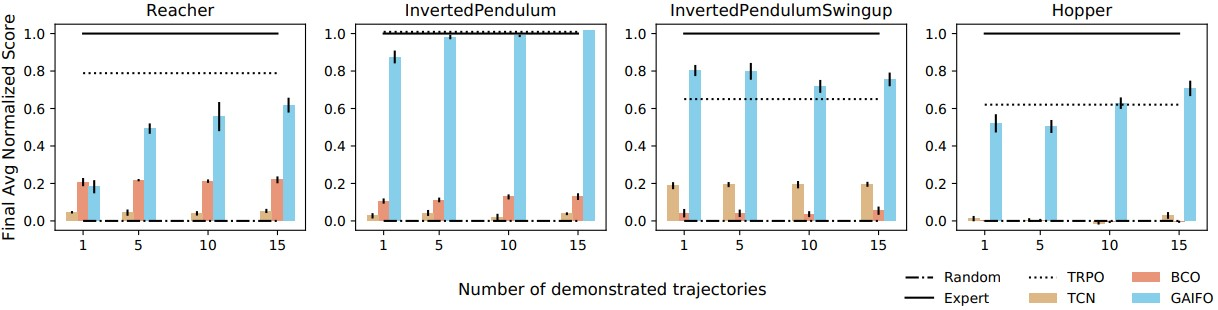
\includegraphics[width=\textwidth]{Figures/images/gaifo_results/gaifo_results_visual.jpg}
         \caption{Experimental results in high-dimensional state space}
         \label{fig:high_dimensional}
     \end{subfigure}
    \hfill
    \caption{Experimental results reported in \cite{torabi2018gaifo}.}
    \label{fig:gaifo_results}
\end{figure}



\paragraph*{Model-Based}\mbox{}\\
Model-Based methods leverage knowledge about the environment dynamics, which is learned through data-driven approaches. These methods can be further classified into \textit{Inverse Dynamic Model} and \textit{Forward Dynamic Model} approaches. 

The \textit{Inverse Dynamic Model} approach, given a transition $(s_{t}, s_{t+1})$, obtains a function $M$ that maps state transitions to actions, i.e., $a_{t} = M(s_{t}, s_{t+1})$. In contrast, the \textit{Forward Dynamic Model} approach, given a state-action pair $(s_{t}, a_{t})$, aims to learn a function $F$ that generates the next state $s_{t+1}$, i.e., $s_{t+1} = F(s_{t}, a_{t})$.

\textbf{Inverse Dynamic Model} methods include \cite{nair2017combining,torabi2018bco,guo2019hybrid_rl,radosavovic2021state_only_demo}.

In \cite{nair2017combining}, the goal was to develop a system capable of tying a knot in a rope. A self-supervised learning approach was used to train a Convolutional Neural Network. Given a pair of images $(I_{t}, I_{t+1})$ representing two successive rope states, the network was able to determine the action required to transition from state $I_{t}$ to state $I_{t+1}$. The network was trained using a dataset of 30K tuples $(I_{t}, a_{t}, I_{t+1})$ collected via an exploratory policy.

Authors in \cite{torabi2018bco} proposed a general approach, depicted in Figure \ref{fig:bco}, composed of two main parts: the learned Inverse Dynamic Model, $M_{\theta}$, and the learned policy $\pi_{\phi}$. The learning procedure is iterative. The model $M_{\theta}^{i}$ is updated by maximizing the probability $p_{\theta}(a_{t}|s_{t}, s_{t+1})$, using tuples $(s_{t}, a_{t}, s_{t+1})$ collected by the current policy. Once the dynamic model is updated, it infers the action $\tilde{a}_{t}$ given the demonstrations. The policy, having access to both state and action information, is then trained using classic Behavioral Cloning (BC) by optimizing the policy parameters through maximum-likelihood estimation $\phi^{*} = \underset{\phi}{argmax} \prod_{i=0}^{N} \pi^{L}_{\phi}(\tilde{a}_{i}|s_{i})$.

In \cite{guo2019hybrid_rl}, a similar approach to \cite{torabi2018bco} was used, but the agent's policy was trained using a combination of Behavioral Cloning and the Advantage Actor Critic (A2C) objective function \cite{mnih2016a2c} (Formula \ref{eq:a2c_reward}).
\begin{equation}
    \label{eq:a2c_reward}
    \begin{aligned}
        \mathcal{L}^{hyb}_{\theta} = \mathbb{E}_{s,a} \left[ A(s)\log(a|s;\theta) + \alpha \ \mathcal{H}(\pi^{L}(.|s)) \right] 
        + \\ \mathbb{E}_{(\hat{s}_{t}, \hat{s}_{t+1}) \sim D} \left[ \log(\pi^{L}(M(\hat{s}_{t}, \hat{s}_{t+1})|\theta)) \right].
    \end{aligned}
  \end{equation}
The main drawback is the assumption of access to the reward function, which can limit its applicability in real-robot manipulation tasks.

In \cite{radosavovic2021state_only_demo}, the work in \cite{Rajeswaran18_learning_complex_dexterous} was extended to state-only demonstrations, and the \textit{State-Only Imitation Learning} (SOIL) algorithm was proposed. This method addresses complex dexterous manipulation tasks, such as object reallocation, tool use, in-hand manipulation, and door opening, using a simulated humanoid hand. A neural network representing the Inverse Dynamic Model was trained by minimizing the L2-loss, given the action performed during the policy rollout. The policy was then updated according to the \textit{Demo Augmented Policy Gradient} (DAPG) method \cite{Rajeswaran18_learning_complex_dexterous}, adapted for state-only demonstrations, which follows the gradient updates described by Formula \ref{eq:dapg_updates}.
\begin{equation}
    \label{eq:dapg_updates}
    \begin{aligned}
        g_{SOIL} = g + \lambda_{0} \ \lambda_{1}^{k} \ \sum_{(s_{t}, \tilde{a}_{t}) \in D'} \nabla_{\theta}\log\pi^{L}_{\theta}(\tilde{a}_{t}, s_{t}),
    \end{aligned}
  \end{equation}

where $g$ is the Natural Policy Gradient term. The idea is to leverage the demonstrations at the beginning of the training and then exploit the RL algorithm to improve the behavior. Experiments performed in simulation showed that, compared to pure RL, the proposed method converges faster and produces more human-like behaviors.

\begin{figure}[tb]
    \centering
    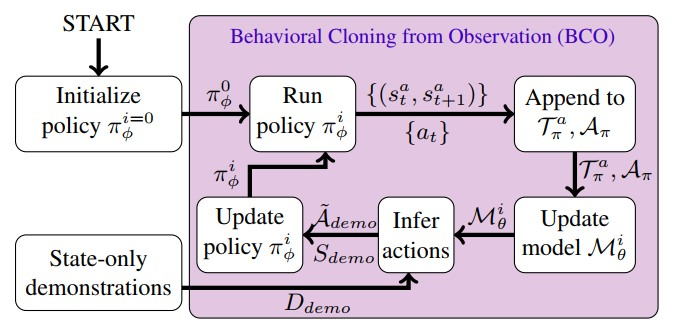
\includegraphics[width=0.6\textwidth]{figures/images/bco/bco.jpg}
    \caption{Representation of the learning procedure proposed by~\cite{torabi2018bco}}
    \label{fig:bco}
\end{figure}


\textbf{Forward Dynamic Model} methods include \cite{smith2019avid,torabi2021dealio}.

In \cite{smith2019avid}, once the human video demonstration was translated into the corresponding robot video, the policy was learned to use the model-based RL algorithm SOLARIS \cite{zhang2019solar}. This algorithm optimizes a controller using the Linear-Quadratic Regulator (LQR) procedure. The policy optimization occurs in a low-dimensional, highly regularized \textit{latent space}, generated using Variational Inference \cite{Kingma2014_vae}. Starting from a sequence of observations and actions, a Global Dynamic Model over the latent trajectory is obtained. Then, given the Latent Dynamic Model, a Linear-Gaussian Controller is derived using LQR-FLM \cite{levine2014lqr_flm}. Real-world robotic experiments demonstrated that with just \textbf{2 hours} of robot interaction, it was possible to outperform previous works such as \cite{sermanet2018time_contrastive,torabi2018bco} and classic BC algorithms in tasks like "coffee making" (Figure \ref{fig:embo_mismatch}) and cup-retrieving, where the robot retrieves a cup from a closed drawer.

In \cite{torabi2021dealio}, the sample inefficiency problem of GAIfO \cite{torabi2018gaifo} was addressed. The approach combined the adversarial learning setting with state-only demonstrations, which had shown promising results (Figure \ref{fig:gaifo_results}), with a more data-efficient RL algorithm like PILQR \cite{chebotar2017pilqr}. PILQR's core is the LQR optimization procedure. Generally, it returns a \textit{linear-gaussian controller} (Formula \ref{formula:linear_gaussian_controller}) that optimizes a \textit{quadratic-cost function} (Formula \ref{formula:quadratic_cost_function}) under the assumption of \textit{linear-gaussian dynamics} (Formula \ref{formula:gaussian_dyn}).

\begin{equation}
\label{formula:linear_gaussian_controller}
    \pi(a_{t}|s_{t}) = \mathcal{N}(K_{t}s_{t} + k_{t}, S_{t})
\end{equation}

\begin{equation}
\label{formula:quadratic_cost_function}
c(s_{t},a_{t}) = \begin{bmatrix}
s_{t}
\\ 
a_{t}
\end{bmatrix}^{T}C_{t}\begin{bmatrix}
s_{t}
\\ 
a_{t}
\end{bmatrix} + \begin{bmatrix}
s_{t}
\\ 
a_{t}
\end{bmatrix}^{T} c_{t} + cc_{t}
\end{equation}

\begin{equation}
\label{formula:gaussian_dyn}
s_{t+1} \sim P(s_{t+1}|s_{t},a_{t}) = \mathcal{N}(F_{t}
\begin{bmatrix}
s_{t}
\\ 
a_{t}
\end{bmatrix} + f_{t}, \Sigma_{t})
\end{equation}




To use this framework, the linear-gaussian dynamic model was fitted using the current policy rollouts. Then, to obtain a quadratic cost function as needed by LQR, the dynamic model was used to express the modified discriminator output (Formula \ref{formula:output_discriminator}) as a function of the pair $(s_{t}, a_{t})$.

\begin{equation}
\label{formula:output_discriminator}
D_{\theta}(s_{t},s_{t+1}) = \frac{1}{2}
\begin{bmatrix}
s_{t}
\\ 
s_{t+1}
\end{bmatrix}^{T}C^{ss}(s_{t},s_{t+1})
\begin{bmatrix}
s_{t}
\\ 
s_{t+1}
\end{bmatrix} + \begin{bmatrix}
s_{t}
\\ 
s_{t+1}
\end{bmatrix}^{T} c^{ss}(s_{t}, s_{t+1})
\end{equation}

Experiments performed in simulation with low-dimensional state spaces showed promising results (Figure \ref{fig:dealio_performance}) in terms of sample efficiency compared to the GAIfO baseline. However, improvements are needed to:
\begin{enumerate*}[label=\textbf{(\arabic*)}]
    \item Reduce variance to make the learning process more reliable,
    \item Increase overall performance,
    \item Adapt the algorithm for real-world robot manipulation tasks.
\end{enumerate*}

\begin{figure}[t]
    \centering
    \begin{subfigure}[b]{0.8\textwidth}
        \centering
        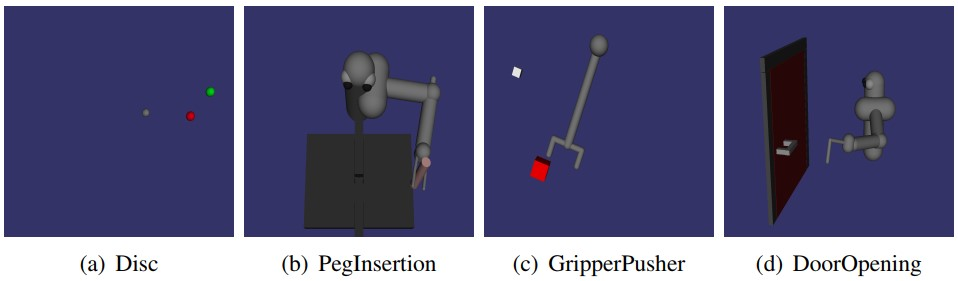
\includegraphics[width=\textwidth]{Figures/images/dealio/dealio_performed_task.jpg}
        \caption{Control Tasks solved in~\cite{torabi2021dealio}}
        \label{fig:dealio_task}
    \end{subfigure}
    \vfill
    \begin{subfigure}[b]{0.8\textwidth}
        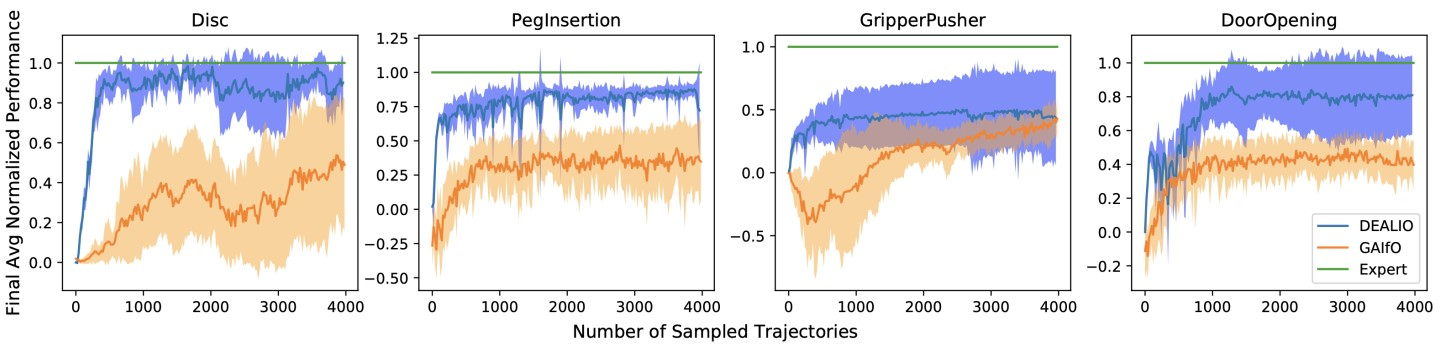
\includegraphics[width=\textwidth]{Figures/images/dealio/dealio_performance.jpg}
        \caption{Performance of DEALIO~\cite{torabi2021dealio} compared against GAIfO~\cite{torabi2018gaifo}, with respect to the number of trajectories sampled during the learning process.}
        \label{fig:dealio_performance}
    \end{subfigure}
    \caption{DEAILO: (\ref{fig:dealio_task}) Control Tasks, (\ref{fig:dealio_performance}) Performance Level}
    \label{fig:dealio}
\end{figure}


Generally, LfO methods have demonstrated interesting features, such as generating a policy from state-based information alone. This supports the hypothesis that the primary source of information for task learning is the sequence of state transitions. Extrapolating the valuable information to perform actions that induce the desired behavior may not be trivial, especially if the state space is represented by images of a human operator. This complexity leads to the design of architectures composed of different stages, which not only increase the complexity of the system itself but also the amount and diversity of data required for their training. Furthermore, many methods of interest have been tested in simulated or relatively simple scenarios, still leaving open whether these methods can be used in real-world complex robotic manipulation tasks.
